\documentclass[10pt, aspectratio=169]{beamer}

\usetheme[progressbar=frametitle]{metropolis}
\usefonttheme{serif}
\setbeamertemplate{frame numbering}[none]
\useoutertheme{metropolis}
\useinnertheme{metropolis}
\usecolortheme{beaver}
\setbeamercolor{background canvas}{bg=white}

\usepackage[italian]{babel}
\usepackage[utf8]{inputenc}
% \usepackage[dvipsnames]{xcolor}
\usepackage{multicol}
\usepackage{mathtools}
\usepackage{parskip}[5pt]
% \usepackage{xcolor}
\definecolor{mypink1}{rgb}{0.858, 0.188, 0.478}



\title{I Prodotti Notevoli}
\subtitle{Dispensa riassuntiva per le classi prime e seconde}
\date{\today}
\author{\em prof. Diego Fantinelli}
\institute{ITET Pasini - Schio}

\titlegraphic{\hfill
\includegraphics[height=12mm]{Pasini_logo.jpeg}}

\begin{document}
\metroset{block=fill}



\maketitle
% \begin{frame}
% 	\titlepage
% \end{frame}



\begin{frame}{indice}
    % \setbeamertemplate{section in toc}[sections numbered]
	\tableofcontents
\end{frame}

\section{I Prodotti Notevoli}

\begin{frame}{Introduzione}
    \begin{alertblock}{definizione}
        \vspace*{10pt}
        \large{ 
        \begin{itemize}
            \item I \textbf{Prodotti Notevoli} sono formule (\textit{espressioni algebriche}), di calcolo che permettono di sviluppare velocemente determinate potenze e prodotti tra polinomi, e viceversa di scomporre determinati tipi di polinomi.
            \item Tali regole vengono chiamate prodotti notevoli perché si riferiscono a prodotti ricorrenti nel calcolo polinomiale.
        \end{itemize}

        }
        \vspace*{10pt}
    \end{alertblock}
    
\end{frame}


% =========================================== somma per differenza

\subsection{Somma per differenza}

\begin{frame}{Somma per differenza}
    % \frametitle{Somma per differenza}
    \begin{columns}
        
        \begin{column}{0.5\textwidth}
            \Large{$$ (A+B)(A-B) = A^2 - B^2$$}
        \end{column}

        \begin{column}{0.5\textwidth}
        {\textbf{Prodotto della somma fra due monomi per la loro differenza}}\\[10pt]

        \small{Consideriamo due monomi, $A$ e $B$, e i binomi che otteniamo dalla loro somma e dalla loro differenza: $A+B$ e $A-B$.\\
        Eseguiamone il prodotto: $(A+B)(A-B)=A^2-A B+A B-B^2=A^2-B^2$\\ [10pt]
        Quindi:}
$$
(A+B)(A-B)=A^2-B^2
$$

        \end{column}
    \end{columns}
\end{frame}

\begin{frame}
    \frametitle{Esempio e note}

    In generale, il prodotto tra la somma di due monomi e la loro differenza è uguale al quadrato del primo termine meno il quadrato del secondo termine. \\[10pt]
\textbf{esempio}:
\hrule

$$\left(2 a^2+3 b^3\right)\left(2 a^2-3 b^3\right)=(\underbracket{2 a^2}_{A})^2- (\underbracket{3 b^3}_{B})^2=4 a^4-9 b^6$$\\[10pt]

Nel precedente esempio e in riferimento alla formula generale $(A+B)(A-B)=A^2-B^2$, abbiamo:

\[
\begin{rcases*}
    A = 2a^2\\
    B= 3b^3
\end{rcases*} \quad \small{\textit{suggerimento: i segni dei due termini non condizionano il risultato}} 
\]


\end{frame}


% =========================================== quadrato di binomio 

\subsection{Quadrato di binomio}

\begin{frame}
    \frametitle{Quadrato di binomio}
    \begin{columns}
        
        \begin{column}{0.5\textwidth}
            \Large{$$ (A+B)^2 = A^2 + 2AB + B^2$$}
        \end{column}

        \begin{column}{0.5\textwidth}
        {\textbf{Quadrato di un binomio}}\\[10pt]
        
        \footnotesize{Consideriamo il binomio $A+B$, in cui $A$ e $B$ rappresentano due monomi e analizziamo che cosa succede moltiplicando il binomio per se stesso, $(A+B)(A+B)=(A+B)^2$. Svolgendo i calcoli si ottiene:}
\begin{flalign*}
    (A+B)^2 & =(A+B)(A+B) = \\ & = A^2+A B+B A+B^2  =A^2+2 A B+B^2
\end{flalign*}
    
Pertanto, senza effettuare i passaggi intermedi si ha
$$
(A+B)^2=A^2+2 A B+B^2
$$
Quindi, il quadrato di un binomio è uguale alla somma algebrica tra il quadrato del primo termine, il quadrato del secondo termine e il doppio prodotto del primo termine per il secondo.
        \end{column}
    \end{columns}
\end{frame}

\begin{frame}
    \frametitle{Esempio e note}

    Eseguendo i prodotti, bisogna fare attenzione ai segni dei monomi: mentre i due quadrati saranno \textbf{sempre positivi}, \em{il doppio prodotto può cambiare segno} a seconda del segno di $A$ e $B$ \\[10pt]
\textbf{esempio}:
\hrule

$$\left(2 a b^3+3 c x\right)^2=4 a^2 b^6+9 c^2 x^2+12 a b^3 c x $$\\ 
mentre:\\
$$  \left(2 a b^3-3 c x\right)^2=4 a^2 b^6+ 9 c^2 x^2-12 a b^3 c x$$

\end{frame}

% =========================================== quadrato di trinomio 

\subsection{Quadrato di un trinomio}

\begin{frame}{Quadrato di trinomio}
    \begin{columns}
        
        \begin{column}{0.5\textwidth}
            \large{

                \begin{flalign*}
                    (A+B+C)^2  = \\ 
                    =A^2+B^2+C^2+2 A B+2 B C+2 A C
                \end{flalign*}
                }

        \end{column}

        \begin{column}{0.5\textwidth}
        {\textbf{Quadrato di un trinomio}}\\[10pt]
        
        {\footnotesize In modo del tutto analogo, considerando il trinomio $A+B+C$, il suo quadrato sarà uguale a:
        $$
        (A+B+C)^2=A^2+B^2+C^2+2 A B+2 B C+2 A C
        $$}\\[20pt]

        \textbf{nota}: Ancora una volta, fare attenzione ai segni quando si eseguono i doppi prodotti
        \end{column} 
    \end{columns}
    
\end{frame} 
            
\begin{frame}{Esempio e note}
\textbf{esempio}:
\hrule
\large{

    \vspace{20pt}
    $$\left(2 a+b^2-x^3 y\right)^2 = 4 a^2+b^4+x^6 y^2+4 a b^2-4 a x^3 y-2 b^2 x^3 y $$
    }

\end{frame}


% =========================================== cubo di binomio 

\subsection{Cubo di un binomio}

\begin{frame}{Cubo di un binomio}
    \begin{columns}
        
        \begin{column}{0.5\textwidth}
            \Large{$$(A+B)^3=A^3+3 A^2 B+3 A B^2+B^3$$}
        \end{column}

        \begin{column}{0.5\textwidth}
        {\textbf{Cubo di un binomio}}\\[10pt]
        
        \footnotesize{Ora eseguiamo il cubo di un binomio: $(A+B)^3=(A+B)(A+B)^2=$ $(A+B)\left(A^2+2 A B+B^2\right)=A^3+2 A^2 B+A B^2+A^2 B+2 A B^2+B^3$ che raccogliendo $\mathrm{i}$ termini simili è uguale a $A^3+3 A^2 B+3 A B^2+B^3$.\\
        In definitiva:}
\begin{flalign*}
    (A+B)^3=A^3+3 A^2 B+3 A B^2+B^3
\end{flalign*}

\vspace{10pt}

\em{Possiamo dunque dire che il cubo di un binomio è uguale alla somma algebrica tra il cubo del primo termine, il cubo del secondo termine, il triplo prodotto del quadrato del primo termine per il secondo termine e il triplo prodotto del primo termine per il quadrato del secondo termine.}
\end{column}

    \end{columns}
\end{frame}

\begin{frame}{Esempio e note}
\textbf{esempio}:
\hrule

\vspace{10pt}

$\begin{aligned}\left(2 a-b^2\right)^3 & =\left(2 a+\left(-b^2\right)\right)^3= \\ & =8 a^3+3 \cdot(2 a)^2 \cdot\left(-b^2\right)+3 \cdot(2 a) \cdot\left(-b^2\right)^2+\left(-b^2\right)^3= \\ & =8 a^3-12 a^2 b^2+6 a b^4-b^6
\end{aligned}$

\end{frame}

% =========================================== somma o differenza di cubi 

\subsection{Somma o differenza di cubi: falso quadrato}

\begin{frame}{Somma o differenza di cubi - \em{falso quadrato}}
    \begin{columns}
        
        \begin{column}{0.5\textwidth}
            \large{$$A^3+B^3=(A+B)\left(A^2-A B+B^2\right) $$}
            \large{$$A^3-B^3=(A-B)\left(A^2+A B+B^2\right) $$}
        \end{column}

        \begin{column}{0.5\textwidth}
        {\textbf{Somma o differenza di cubi}}\\[10pt]
        
        \footnotesize{Ora eseguiamo il seguente prodotto:
        \begin{flalign*}
            & (A+B)\left(A^2-A B+B^2\right)  =\\ 
            & = A^3-A^2 B+A^2 B+A B^2-A B^2+B^3\\ 
            & =A^3+B^3
        \end{flalign*}
        
        Il trinomio $A^2-A B+B^2$ è comunemente noto come falso quadrato, poiché differisce da quadrato di un binomio solo per il fattore $2$.\\
        Leggendo la catena di uguaglianze nell'altro verso, possiamo concludere che
        $$
        A^3+B^3=(A+B)\left(A^2-A B+B^2\right)
        $$
        Con calcoli del tutto analoghi, si conclude che
        $$
        A^3-B^3=(A-B)\left(A^2+A B+B^2\right)
        $$}

    
        \end{column}
    \end{columns}
\end{frame}

\begin{frame}
    \frametitle{Esempio e note}

    Notare come il segno presente nel falso quadrato sia l'opposto di quello tra i due cubi, mentre il segno presente nel binomio sia invece lo stesso. \\[10pt]
\textbf{esempio}:
\hrule

\begin{flalign*} 
    8 a^6-27 b^3 & =\left(2 a^2\right)^3-(3 b)^3= \\ & =\left(2 a^2-3 b\right)\left(\left(2 a^2\right)^2+2 a^2 \cdot 3 b+(3 b)^2\right)= \\ & =\left(2 a^2-3 b\right)\left(4 a^4+6 a^2 b+9 b^2\right)
\end{flalign*}

\vspace*{20pt}

\em{Questo Prodotto Notevole è "meno famoso" degli altri, perchè viene utilizzato di meno, ma quando $i$ calcoli si faranno più complessi - soprattutto all'Università -  ricordarlo vi farà risparmiare un sacco di tempo e, in un esame, il tempo è preziosissimo.}
\end{frame}

\section{Conclusioni}

\begin{frame}[t]{Conclusioni}
    \vspace{2cm}
    
        \large { \textcolor{purple}{I Prodotti Notevoli non sono altro che dei casi particolari di moltiplicazioni tra Polinomi che vengono utilizzati molto spesso nel Calcolo Letterale, quindi conviene \em{impararli a memoria}; ma la cosa fondamentale è che vanno letti, utilizzati e imparati, \textbf{in entrambe le direzioni!} dell'uguaglianza:\\[20pt]
        \begin{itemize}
            \item da sinistra a destra avrete dei \textbf{prodotti notevoli}
            \item da destra a sinistra avrete delle \textbf{scomposizioni di polinomi}
        \end{itemize}}}

\end{frame}

\definecolor{mypink2}{RGB}{219, 48, 122}
\definecolor{mypink3}{cmyk}{0, 0.7808, 0.4429, 0.1412}
\definecolor{mygray}{gray}{0.6}

\setbeamertemplate{background} 
{
    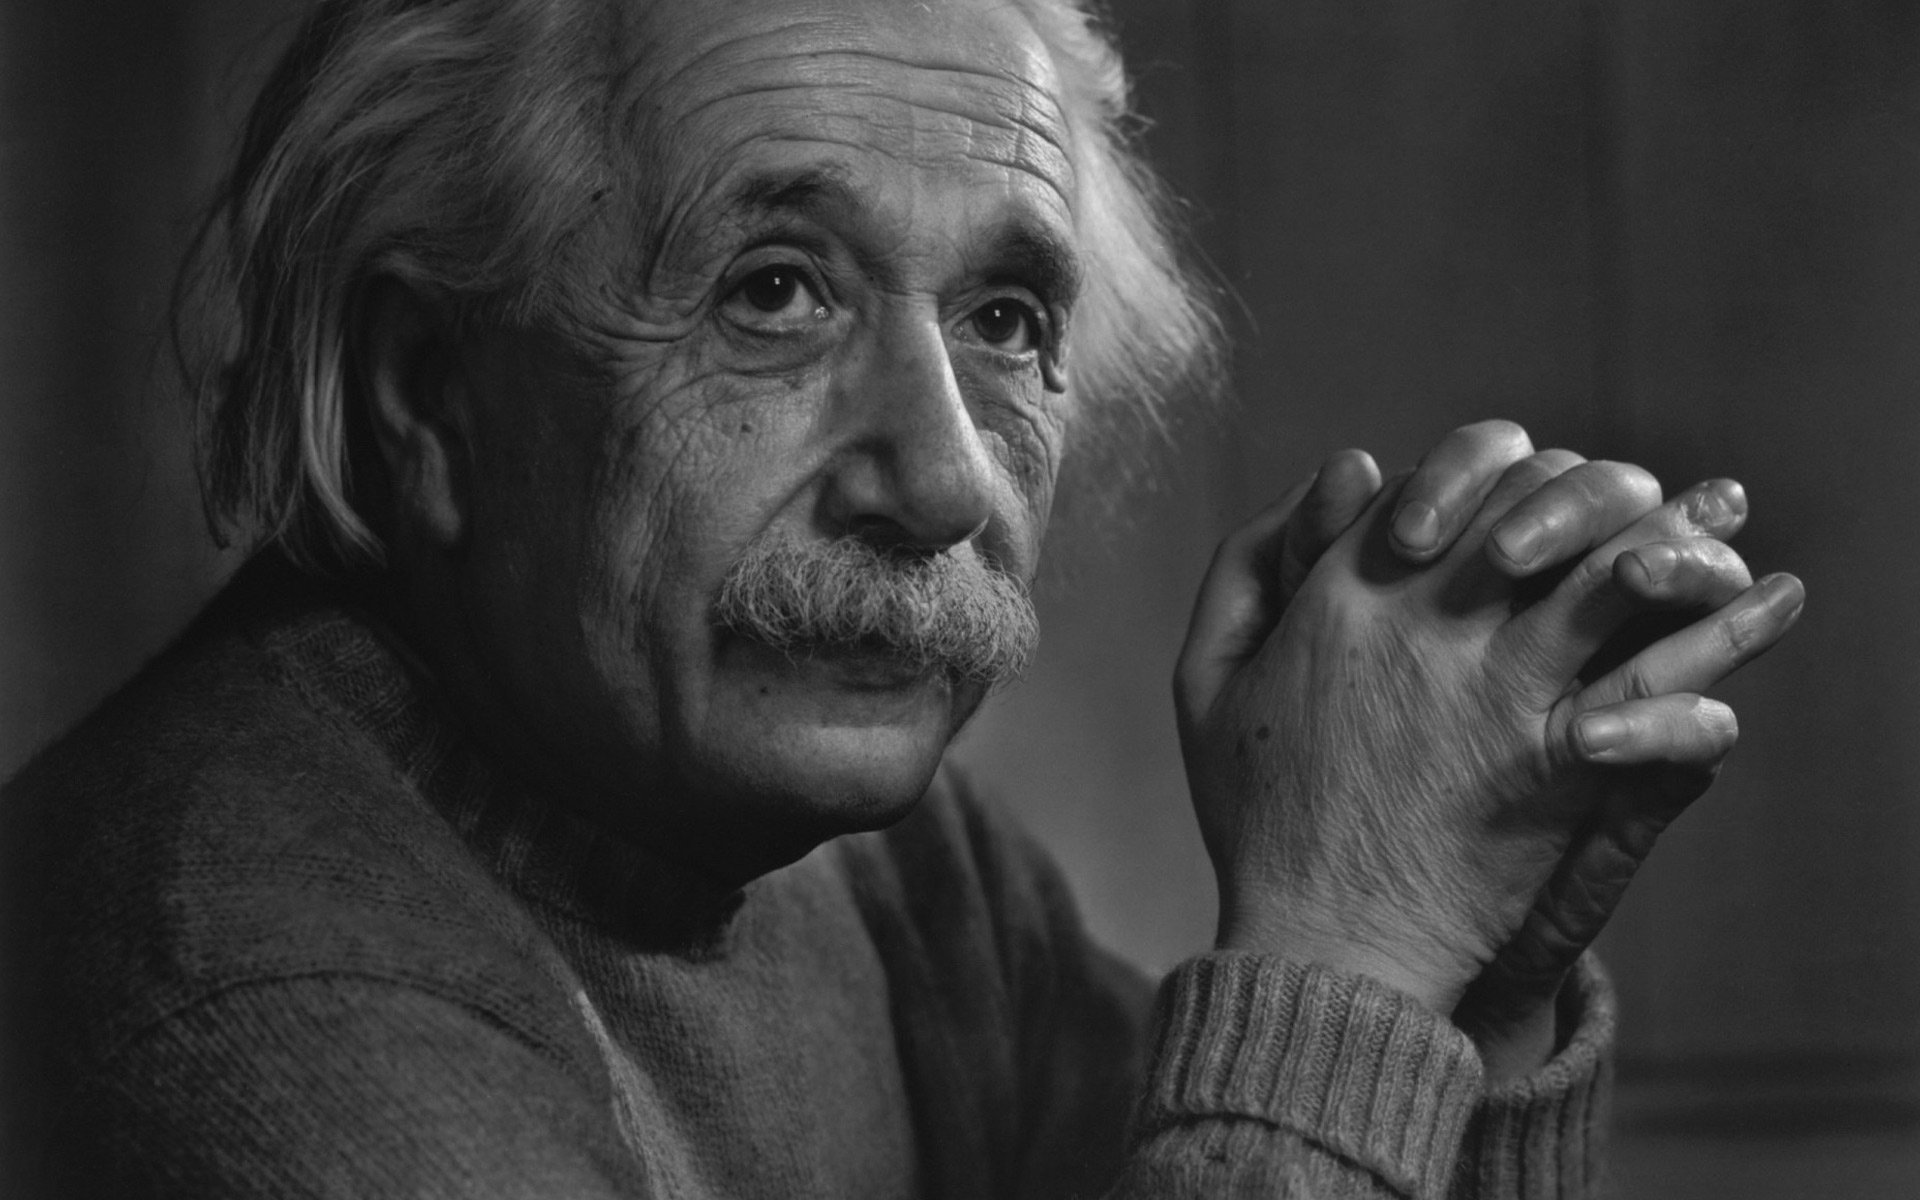
\includegraphics[width=\paperwidth,height=\paperheight]{ae.jpeg}
}
{\setbeamercolor{palette primary}{fg=black, bg=mypink3}
\begin{frame}[standout]
    \LARGE {\textit{ \textcolor{white}{“Non hai veramente capito qualcosa fino a quando non sei in grado di spiegarlo a tua nonna”\\[20 pt]
    (A. Einstein)}}}

    % 
\includegraphics[scale=0.2]{einstein.png}
\end{frame}
}


\end{document}